\documentclass{standalone}
\usepackage{tikz}

\begin{document}
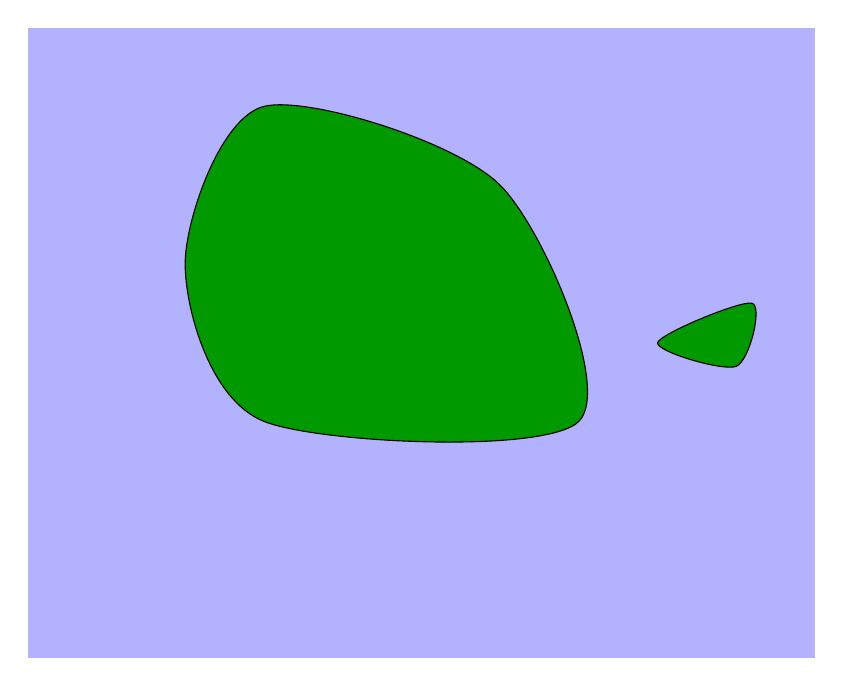
\begin{tikzpicture}
    % desenhando o país
    \draw[fill=green!60!black] plot[smooth cycle] coordinates {(0,0) (4,0) (3,3) (0,4) (-1,2)};
    % desenhando a ilha
    \draw[fill=green!60!black] plot[smooth cycle] coordinates {(5,1) (6,0.7) (6.2, 1.5)};
    % desenhando o mar
    \fill[blue!30] (-3,-3) rectangle (7,5);
    % redesenhando o país e a ilha por cima do mar
    \draw[fill=green!60!black] plot[smooth cycle] coordinates {(0,0) (4,0) (3,3) (0,4) (-1,2)};
    \draw[fill=green!60!black] plot[smooth cycle] coordinates {(5,1) (6,0.7) (6.2, 1.5)};
\end{tikzpicture}
\end{document}